\chapter{Method}

Pragmatism == Usefulness/Utility => Truth

% Idea: ``Can I add a bit of code, that sidesteps frameworks, and talks to all plutt app, to fetch and distribute shared assets?''

% This idea would be stronger if asset management was automatic. A centralized tool could decide if an asset should be bundled or separate.

\section{Artifacts (Contributions)}
What are my artifacts?
\begin{itemize}
    \item constructs: 
    \item models:
    \item methods:
    \item instantiations:
\end{itemize}

\section{Guidelines}

This whole section is based on \cite{Hevner2004}

\begin{enumerate}
    \item \textbf{Design as an artifact:} Design-science research must produce a viable artifact in the form of a construct, a model, a method, or an instantiation.
    \item \textbf{Problem relevance:} The objective of design-science research is to develop technology-based solutions to important and relevant business problems.
    \item \textbf{Design evaluation:} The utility, quality, and efficacy of a design artifact must be rigorously demonstrated via well-executed evaluation methods.
    \item \textbf{Research contributions:} Effective design-science research must provide clear and verifiable contributions in the areas of the design artifact, design foundations, and/or design methodologies.
    \item \textbf{Research rigor:} Design-science research relies upon the application of rigorous methods in both the construction and evaluation of the design artifact.
    \item \textbf{Design as a search process:} The search for an effective artifact requires utilizing available means to reach desired ends while satisfying laws in the problem environment.
    \item \textbf{Communication of research:} Design-science research must be presented effectively both to technology-oriented as well as management-oriented audiences.
\end{enumerate}


\subsection{Guideline 1: Design as an artifact}
The purpose is to create an artifact. This is defined in section artifacts.

\subsection{Guideline 2: Problem Relevance}
\textit{The objective of design technology-based solutions is to develop important and relevant business problems.}

\textbf{Define what the problem is and why it is relevant.}

The problem in a general context is that companies that would like to try, evaluate or migrate to \ac{MFE} architecture, have to do large changes to their codebase to reap any rewards. They sometimes have to align large parts of the company to move in that direction at the same time, giving an organizational challenge. The technology to try out \ac{MFE} does exist with web components, but they come with other problems, and should be migrated away from.

The specific evaluation context is that DigitalRoute would like to try out \acp{MFE} but does not want to rewrite large parts of their \ac{FE}. They are going to add a new team soon who will be responsible for a part of the \ac{FE}. This part could be included into the main web page using \ac{MFE} technologies.

\subsection{Guideline 3: Design Evaluation}
\textit{The utility, quality, and efficacy of a design artifact must be rigorously demonstrated via well-executed evaluation methods.}

\textit{Thus, evaluation includes the integration of the artifact within the technical infrastructure of the business environment.}

\textit{IT artifacts can be evaluated in terms of functionality, completeness, consistency, accuracy, performance, reliability, usability, fit with the organization, and other relevant quality attributes}

\textit{A design artifact is complete and effective when it satisfies the requirements and constraints of the problem it was meant to solve.}

\textbf{What are the requirements and constraints of the problem it was meant to solve?}
The artifact has to be easy to include in an existing project, with little to no changes to the original code base. Also it has to be adapted to enable typical \ac{MFE} advantages, like asynchronous releases and team independence (especially as their will be a very remote team handling the \ac{MFE} fragments).

\textit{... descriptive methods of evaluation should only be used for especially innovative artifacts for which other forms of evaluation may not be feasible.}

\textbf{Using FEDS:}

\textbf{Why to evaluate? Formative vs summative evaluation:} Formative is \textit{categorical} and future while summative is \textit{continous} and looking at the performance of something that has happened.

\textbf{When to evaluate: ex ante vs ex post evaluation:} Am I addressing a specific system (new of artifact) or a specific problem (new kind of problem).

\textbf{Why to evaluate: purpose and goals of evaluation in DSR}
6 different purposes

\textbf{Problems with evaluation}
False positives and false negatives. Maybe I evaluate that the artifact does not work when it actually does. Or the opposite.

\begin{figure}[!ht]
    \centering
    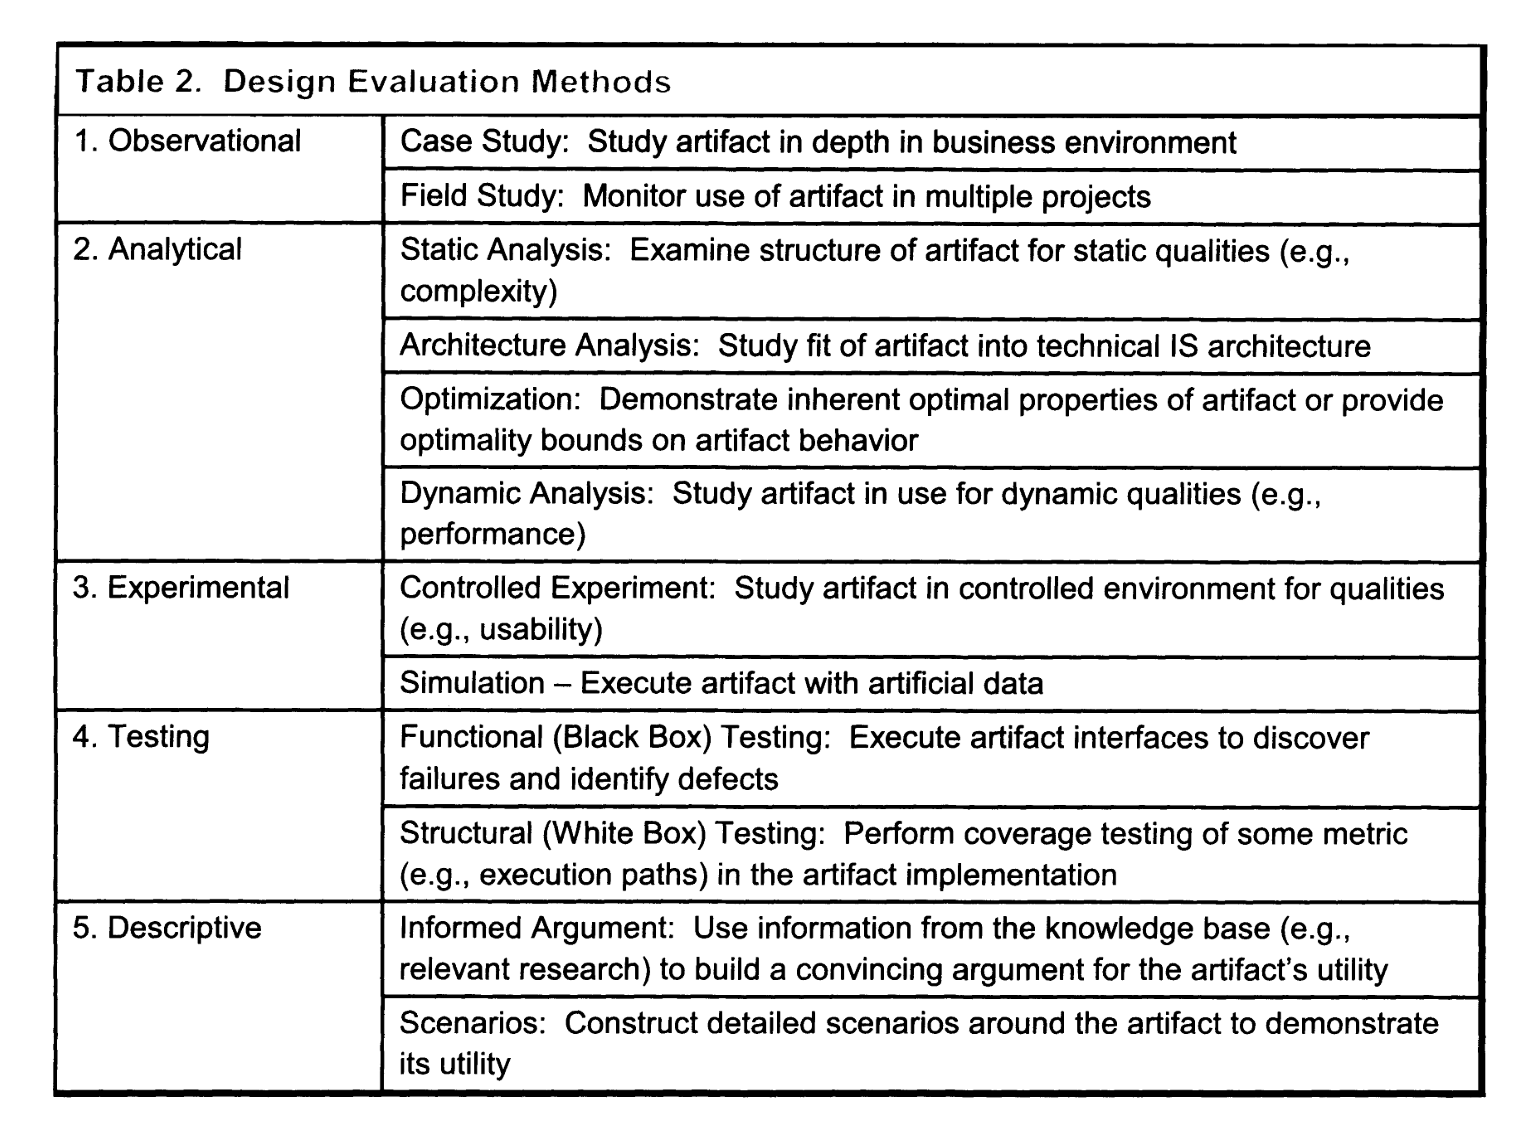
\includegraphics[width=\textwidth]{images/copy-temp.png}
    \caption{Copy from \cite{Hevner2004}}
\end{figure}

\subsection{Guideline 4: Research Contributions}
\textit{Effective design-science research must provide clear and verifiable contributions in the areas of the design artifact, design foundations, and/or design methodologies.}

Is the contribution the artifact, or foundational knowledge? If it is the artifact it has to do the following:
\textit{The artifact must enable the solution of heretofore unsolved problems. It may extend the knowledge base (see below) or apply existing knowledge in new and innovative ways.}

If it is foundational knowledge it has to do the following:
\textit{The creative development of novel, appropriately evaluated constructs, models, methods, or instantiations that extend and improve the existing foundations in the design-science knowledge base are also important contributions.}

\subsection{Guideline 5: Research Rigor}
\textit{In both design-science and behavioral-science research, rigor is derived from the effective use of the knowledge base?theoretical foundations and research methodologies. Success is predicated on the researcher's skilled selection of appropriate techniques to develop or construct a theory or artifact and the selection of appropriate means to justify the theory or evaluate the artifact.}

This can be done by evaluating (not implementing) the artifacts from multiple contexts (Like react, vue, angular).

\textit{Design-science researchers must constantly assess the appropriateness of their metrics and the construction of effective metrics is an important part of design-science research.}

\subsection{Guideline 6: Design as a Search Process}
Iterative process.

\subsection{Guideline 7: Communication of Research}
Repeatability. Explain clearly what was done and how, like relevant implementation details.

\textit{That is, the emphasis must be on the importance of the problem and the novelty and effectiveness of the solution approach realized in the artifact.}